\documentclass[11pt,oneside]{book}

% ============================================================================
% PACKAGES & TYPOGRAPHY
% ============================================================================
\usepackage[utf8]{inputenc}
\usepackage[T1]{fontenc}
\usepackage{lmodern}
\usepackage{microtype}
\usepackage[a4paper,margin=2.2cm,headheight=15pt]{geometry}
\usepackage{xcolor}
\usepackage{amsmath,amssymb}
\usepackage{booktabs}
\usepackage{longtable}
\usepackage{tabularx}
\usepackage{array}
\usepackage{enumitem}
\usepackage{fancyhdr}
\usepackage{titlesec}
\usepackage{tikz}
\usetikzlibrary{arrows.meta,positioning,shapes.geometric,calc,fit,backgrounds}
\usepackage{listings}
\usepackage[most]{tcolorbox}
\usepackage[colorlinks=true,linkcolor=NavyBlue,urlcolor=TealBlue,citecolor=NavyBlue]{hyperref}

% ============================================================================
% COLOR PALETTE (FSDG / GNU Engineering Theme)
% ============================================================================
\definecolor{NavyBlue}{HTML}{0B3C5D}
\definecolor{TealBlue}{HTML}{0F6B78}
\definecolor{CrimsonRed}{HTML}{8E1600}
\definecolor{AmberGold}{HTML}{B86B00}
\definecolor{ForestGreen}{HTML}{1B5E20}
\definecolor{SlateGray}{HTML}{2C3E50}
\definecolor{CodeBg}{HTML}{F7F9FB}
\definecolor{CodeFrame}{HTML}{D0D7DE}
\definecolor{CommentGreen}{HTML}{2E7D32}
\definecolor{StringPurple}{HTML}{6A1B9A}

% ============================================================================
% HEADERS & CHAPTER STYLING
% ============================================================================
\pagestyle{fancy}
\fancyhf{}
\fancyhead[L]{\nouppercase{\leftmark}}
\fancyhead[R]{\thepage}
\renewcommand{\headrulewidth}{0.4pt}

\titleformat{\chapter}[display]
  {\normalfont\huge\bfseries\color{NavyBlue}}
  {\filright\normalsize\color{TealBlue}\MakeUppercase{\chaptertitlename}\ \thechapter}
  {8pt}
  {\titlerule[1.2pt]\vspace{6pt}\filright}
  [\vspace{4pt}\titlerule]

\setlength{\parskip}{0.45em}
\setlength{\parindent}{0pt}

% ============================================================================
% LISTINGS CONFIGURATION (Guile Scheme, Emacs Lisp, Org-Mode, Bash)
% ============================================================================
\lstdefinelanguage{GuileScheme}{
  sensitive=true,
  morecomment=[l]{;},
  morestring=[b]",
  alsoletter={-,?,!,*,+,/,<,>,=,:,#,~,\$,@},
  morekeywords=[1]{
    define,define*,define-public,define-module,use-modules,
    define-record-type,define-record-type*,define-syntax,define-syntax-rule,
    syntax-rules,syntax-case,lambda,case-lambda,let,let*,letrec,let-values,
    define-values,if,cond,case,when,unless,begin,and,or,not,match,
    set!,quote,quasiquote,unquote,unquote-splicing,
    with-imported-modules,gexp,ungexp,ungexp-splicing
  },
  morekeywords=[2]{
    operating-system,home-environment,file-system,mapped-device,
    swap-space,user-account,user-group,bootloader-configuration,
    service,simple-service,modify-services,service-extension,
    shepherd-service,shepherd-action,channel,make-channel-introduction,
    openpgp-fingerprint,package,origin,local-file,plain-file,computed-file,
    file-append,program-file,scheme-file
  },
  morekeywords=[3]{
    #:use-module,#:export,#:re-export,#:prefix,#:select,#:key,#:optional,
    #:rest,#:allow-other-keys,#:recursive?,#:locales,#:name,#:log-file,
    #t,#f,#~,#\$,#\$@
  }
}

\lstdefinelanguage{EmacsLisp}{
  sensitive=true,
  morecomment=[l]{;},
  morestring=[b]",
  alsoletter={-,?,!,*,+,/,<,>,=,:},
  morekeywords=[1]{
    defun,defmacro,defvar,defconst,defcustom,setq,setq-default,
    let,let*,if,when,unless,cond,pcase,dolist,dotimes,while,
    lambda,function,funcall,apply,mapcar,require,provide,
    use-package,with-eval-after-load,condition-case,unwind-protect,
    save-excursion,with-temp-buffer,define-advice,advice-add
  },
  morekeywords=[2]{
    :init,:config,:custom,:hook,:bind,:map,:after,:demand,:ensure,:defer,
    :wk,:ignore,t,nil
  }
}

\lstdefinelanguage{OrgMode}{
  sensitive=false,
  morecomment=[l]{\#},
  morestring=[b]",
  alsoletter={+,:,*,#,<,>,-},
  morekeywords=[1]{
    TODO,NEXT,WAIT,DONE,CANCELLED,PROJ,COMPLETED,SCHEDULED:,DEADLINE:,
    :PROPERTIES:,:END:,:LOGBOOK:,:ID:,:CREATED:,:EFFORT:,:header-args:
  },
  morekeywords=[2]{
    :tangle,:tangle-mode,:mkdirp,:noweb,:results,:session,:var,:exports,:colnames
  }
}

\lstset{
  basicstyle=\ttfamily\small,
  backgroundcolor=\color{CodeBg},
  frame=single,
  rulecolor=\color{CodeFrame},
  framesep=4pt,
  xleftmargin=6pt,
  xrightmargin=6pt,
  breaklines=true,
  breakatwhitespace=false,
  columns=fullflexible,
  keepspaces=true,
  showstringspaces=false,
  keywordstyle=[1]\bfseries\color{NavyBlue},
  keywordstyle=[2]\bfseries\color{TealBlue},
  keywordstyle=[3]\bfseries\color{CrimsonRed},
  commentstyle=\itshape\color{CommentGreen},
  stringstyle=\color{StringPurple},
  upquote=true
}

% ============================================================================
% TCOLORBOX CALLOUT ENVIRONMENTS
% ============================================================================
\newtcolorbox{beginnertip}[1][Beginner Mental Model]{
  enhanced,
  breakable,
  colback=TealBlue!5!white,
  colframe=TealBlue,
  fonttitle=\bfseries,
  title={#1},
  arc=2mm,
  boxrule=0.8pt,
  left=8pt,right=8pt,top=6pt,bottom=6pt
}

\newtcolorbox{protrap}[1][Production Trap \& Post-Mortem]{
  enhanced,
  breakable,
  colback=CrimsonRed!5!white,
  colframe=CrimsonRed,
  fonttitle=\bfseries,
  title={#1},
  arc=2mm,
  boxrule=0.9pt,
  left=8pt,right=8pt,top=6pt,bottom=6pt
}

\newtcolorbox{exercisebox}[1][Hands-On Engineering Lab]{
  enhanced,
  breakable,
  colback=AmberGold!6!white,
  colframe=AmberGold!90!black,
  fonttitle=\bfseries,
  title={#1},
  arc=2mm,
  boxrule=0.8pt,
  left=8pt,right=8pt,top=6pt,bottom=6pt
}

\newtcolorbox{architecturebox}[1][System Architecture Principle]{
  enhanced,
  breakable,
  colback=NavyBlue!5!white,
  colframe=NavyBlue,
  fonttitle=\bfseries,
  title={#1},
  arc=2mm,
  boxrule=0.8pt,
  left=8pt,right=8pt,top=6pt,bottom=6pt
}

% ============================================================================
% DOCUMENT METADATA
% ============================================================================
\title{%
  \vspace{-1cm}
  {\Huge\bfseries\color{NavyBlue} Guile Scheme, GNU Guix, GNU Emacs \& Org-Mode}\\[0.6em]
  {\Large\bfseries\color{TealBlue} The Complete Zero-to-Production Linux Systems Engineering Masterclass}\\[1.2em]
  {\normalsize From S-Expressions, G-Expressions, and PID 1 Shepherd Services to Structural Lisp Editing, Literate Org-Babel OS Tangling, and Fail-Closed Verification Gates}
}
\author{\textbf{Written for Omran ``devo'' Altunaiji}\\Linux / DevOps Systems Engineering Curriculum}
\date{Edition 2026.11 --- FSDG-Compliant Pure GNU Guix Reference}

\begin{document}

\maketitle
\tableofcontents

% ============================================================================
% CHAPTER 1: MODULE 1 — THE LISP MINDSET
% ============================================================================
\chapter{The Lisp Mindset: Demystifying Parentheses, Cons Cells \& Homoiconicity}

\section{Why Prefix S-Expressions Have Zero Operator-Precedence Ambiguity}

Systems engineers coming from C, Bash, Python, or Go initially perceive Lisp code as a dense wall of parentheses. In C or Python, surface syntax relies on infix operators (\texttt{+}, \texttt{*}, \texttt{\&}, \texttt{==}), unary prefixes, and implicit precedence tables (for example, in C \texttt{x \& y == 0} parses as \texttt{x \& (y == 0)}, a notorious source of kernel bugs). When a compiler parses \texttt{a + b * c}, it immediately discards the infix string and constructs an in-memory Abstract Syntax Tree (AST).

In Guile Scheme, \textbf{you write the compiler's AST directly} using Symbolic Expressions (\textbf{S-expressions}):

\begin{lstlisting}[language=GuileScheme]
;; Every parenthesized list in Scheme obeys one universal rule:
;;   (operator operand-1 operand-2 ...)
(+ a (* b c))
(string-append "/home/" user "/.ssh/authorized_keys")
\end{lstlisting}

\begin{itemize}[leftmargin=1.5em]
  \item \textbf{Slot 0 (the head)} is always the operation: a procedure, a macro, or a special form (\texttt{define}, \texttt{let}, \texttt{if}, \texttt{lambda}, \texttt{quote}).
  \item \textbf{Slots 1..N (the tail)} are always the arguments evaluated and passed to that operation.
  \item \textbf{Zero Precedence Rules}: Grouping is explicit and local. Variadic procedures (\texttt{+}, \texttt{string-append}, \texttt{cons*}) take arbitrarily many operands without repeating the operator.
\end{itemize}

\begin{beginnertip}[Reading S-Expressions: Outside-In vs. Inside-Out]
Never count parentheses from left to right. Instead, use two complementary reading modes:
\begin{enumerate}
  \item \textbf{Outside-In (Top-Down Structural Intent)}: Read declarations, \texttt{if}/\texttt{cond} branches, and \texttt{(operating-system ...)} records from the outermost keyword inward, following indentation depth.
  \item \textbf{Inside-Out (Bottom-Up Dataflow)}: Trace nested data transformations from the deepest leaf expression outward, just like a Unix pipeline \texttt{current-filename | or "." | dirname | string-append}:
\end{enumerate}
\begin{lstlisting}[language=GuileScheme]
;; From guix-platform-install/oracle/image/oracle-image.scm:
(string-append (dirname (or (current-filename) ".")) "/authorized-key.pub")
;; 1. (current-filename) => "/root/guix/oracle/image/oracle-image.scm"
;; 2. (or ... ".")       => "/root/guix/oracle/image/oracle-image.scm"
;; 3. (dirname ...)      => "/root/guix/oracle/image"
;; 4. (string-append ..) => "/root/guix/oracle/image/authorized-key.pub"
\end{lstlisting}
\end{beginnertip}

\section{Atoms, Homoiconicity, and Quasiquotation (\texttt{'}, \texttt{`}, \texttt{,}, \texttt{,@})}

Every Scheme form is either an indivisible \textbf{Atom} or a \textbf{Pair/List}. Self-evaluating atoms evaluate to themselves: numbers (\texttt{42}, octal \texttt{\#o700}, hex \texttt{\#x1b}), strings (\texttt{"/gnu/store"}), booleans (\texttt{\#t}, \texttt{\#f}), characters (\texttt{\#\textbackslash newline}, \texttt{\#\textbackslash :}), and keywords (\texttt{\#:use-module}). By contrast, an unquoted \textbf{Symbol} (\texttt{eth0}, \texttt{glibc}) is evaluated as a lexical variable lookup.

Because Scheme source code is represented as Scheme lists, \textbf{code is data and data is code} (\emph{homoiconicity}). Placing a single quote \texttt{'} before a form freezes evaluation and returns the literal AST list:

\begin{lstlisting}[language=GuileScheme]
(+ 1 2)                        ; Evaluates procedure call => 3
'(+ 1 2)                       ; Returns 3-element data list => (+ 1 2)
(list '+ 1 2)                  ; Constructs the exact same list => (+ 1 2)
(equal? '(+ 1 2) (list '+ 1 2)) ; => #t
\end{lstlisting}

When constructing configuration trees or G-expressions that are 90\% static structure and 10\% computed values, Scheme provides \textbf{Quasiquotation} (\texttt{`}), \textbf{Unquote} (\texttt{,}), and \textbf{Unquote-Splicing} (\texttt{,@}), which map 1-to-1 onto GNU Guix \textbf{G-Expressions} (\texttt{\#\textasciitilde}, \texttt{\#\$}, \texttt{\#\$@}):

\begin{center}
\begin{tabularx}{\textwidth}{llllX}
\toprule
\textbf{Scheme} & \textbf{Reader Form} & \textbf{Guix G-Exp} & \textbf{Shell Analogy} & \textbf{Semantics} \\
\midrule
\texttt{'expr} & \texttt{(quote expr)} & --- & \texttt{'literal \$X'} & Freeze entire tree as literal data. \\
\texttt{`expr} & \texttt{(quasiquote expr)} & \texttt{\#\textasciitilde expr} & \texttt{"template \$X"} & Literal data template \emph{except} where unquoted. \\
\texttt{,expr} & \texttt{(unquote expr)} & \texttt{\#\$expr} & \texttt{"\$VAR"} & Evaluate \texttt{expr} now and insert single result. \\
\texttt{,@expr} & \texttt{(unquote-splicing)} & \texttt{\#\$@expr} & \texttt{"\$\{ARR[@]\}"} & Evaluate list \texttt{expr} and splice elements inline. \\
\bottomrule
\end{tabularx}
\end{center}

\section{Cons Cells (\texttt{cons}, \texttt{car}, \texttt{cdr}), Proper Lists \& Structural Sharing}

At the memory level, a Scheme pair is a two-pointer struct allocated by \texttt{(cons a b)} whose first slot is \texttt{car} (\emph{head}) and whose second slot is \texttt{cdr} (\emph{tail}). A \textbf{proper list} \texttt{(a b c)} is a linked spine of cons cells terminated by the empty list \texttt{'()}:

\begin{center}
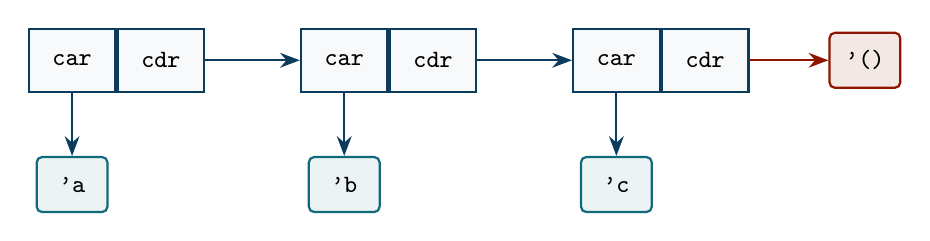
\begin{tikzpicture}[
  cell/.style={draw=NavyBlue,thick,minimum width=1.1cm,minimum height=0.8cm,fill=CodeBg,font=\ttfamily\small},
  atom/.style={draw=TealBlue,thick,rounded corners=2pt,fill=TealBlue!8,minimum width=0.9cm,minimum height=0.7cm,font=\ttfamily\small},
  arrow/.style={-{Stealth[length=2.5mm]},thick,color=NavyBlue}
]
  % Cell 1
  \node[cell] (c1a) at (0,0) {car};
  \node[cell,right=0pt of c1a] (c1d) {cdr};
  \node[atom,below=0.8cm of c1a] (a1) {'a};
  \draw[arrow] (c1a.south) -- (a1.north);

  % Cell 2
  \node[cell,right=1.2cm of c1d] (c2a) {car};
  \node[cell,right=0pt of c2a] (c2d) {cdr};
  \node[atom,below=0.8cm of c2a] (a2) {'b};
  \draw[arrow] (c2a.south) -- (a2.north);
  \draw[arrow] (c1d.east) -- (c2a.west);

  % Cell 3
  \node[cell,right=1.2cm of c2d] (c3a) {car};
  \node[cell,right=0pt of c3a] (c3d) {cdr};
  \node[atom,below=0.8cm of c3a] (a3) {'c};
  \draw[arrow] (c3a.south) -- (a3.north);
  \draw[arrow] (c2d.east) -- (c3a.west);

  % Empty list terminator
  \node[atom,right=1.0cm of c3d,fill=CrimsonRed!10,draw=CrimsonRed] (nil) {'()};
  \draw[arrow,color=CrimsonRed] (c3d.east) -- (nil.west);
\end{tikzpicture}
\end{center}

When you write \texttt{(cons my-user \%base-user-accounts)} in a Guix \texttt{operating-system} declaration, Scheme does \textbf{not} copy \texttt{\%base-user-accounts}. Because lists are treated immutably, \texttt{cons} allocates a single 16-byte cons cell whose \texttt{car} points to \texttt{my-user} and whose \texttt{cdr} shares the existing spine of \texttt{\%base-user-accounts} in $O(1)$ time and space.

\section{Tail-Call Optimization (TCO), Named \texttt{let}, and \texttt{(srfi srfi-1)}}

In Scheme, any procedure call in \textbf{tail position} (the very last operation before returning) is guaranteed by the language standard to execute in $O(1)$ stack space via Tail-Call Optimization. Idiomatic Guile uses \textbf{named \texttt{let}} for state-machine loops (such as retry loops with exponential backoff) and \texttt{(srfi srfi-1)} (\texttt{map}, \texttt{filter}, \texttt{fold}, \texttt{partition}, \texttt{delete-duplicates}) for collection pipelines:

\begin{lstlisting}[language=GuileScheme]
(use-modules (srfi srfi-1))

;; Named `let' compiles to an O(1)-stack jump loop:
(define (retry-with-backoff thunk max-attempts)
  (let loop ((attempt 1)
             (delay-sec 1))
    (let ((result (thunk attempt)))
      (cond
        (result (cons* 'ok attempt result))
        ((>= attempt max-attempts) (list 'failed attempt))
        (else
          (sleep delay-sec)
          (loop (+ attempt 1) (* delay-sec 2)))))))
\end{lstlisting}

% ============================================================================
% CHAPTER 2: MODULE 2 — GUILE SCHEME FOR SYSTEMS ENGINEERS
% ============================================================================
\chapter{Guile Scheme for Systems Engineers}

\section{The Kernel Shebang Limit (\texttt{fs/binfmt\_script.c}) \& Octal Escape Trap}

When the Linux kernel executes a script starting with \texttt{\#!}, \texttt{fs/binfmt\_script.c} splits the first line at the first whitespace after the interpreter path and passes the \textbf{entire remainder of the line as a single argument} (\texttt{argv[1]}). Therefore, \texttt{\#!/usr/bin/env guile -e main -s} fails because \texttt{env} looks for a binary literally named \texttt{"guile -e main -s"}.

Guile solves this with its multi-line \textbf{meta-switch} (\texttt{\textbackslash} at the end of line 1, multi-word flags on line 2, closed by \texttt{!\#} on line 3):

\begin{lstlisting}[language=GuileScheme]
#!/run/current-system/profile/bin/guile \
--no-auto-compile -e main -s
!#
(use-modules (ice-9 format)
             (ice-9 match))

(define (main args)
  ;; CRITICAL: Guile strings have NO octal escape (\033 is NUL + "33"!).
  ;; Always use hexadecimal \x1b for ANSI escape sequences:
  (format #t "\x1b[32m[OK]\x1b[0m Invoked with args: ~s~%" (cdr args)))
\end{lstlisting}

\begin{protrap}[Never Use \texttt{\#!/bin/bash} on GNU Guix Targets]
On a pure GNU Guix System, \texttt{/bin} contains only \texttt{/bin/sh} (for POSIX \texttt{system(3)} compatibility). Bash resides in \texttt{/gnu/store/.../bin/bash} and is linked at \texttt{/run/current-system/profile/bin/bash}. Scripts targeting a booted Guix system must use \texttt{\#!/run/current-system/profile/bin/bash} (or \texttt{.../guile}); portable developer tooling must use \texttt{\#!/usr/bin/env bash}.
\end{protrap}

\section{Guile Modules (\texttt{define-module}) \& Guix Records (\texttt{define-record-type*})}

A Guile module name \texttt{(my-org storage btrfs)} maps directly to the relative filesystem path \texttt{my-org/storage/btrfs.scm} along \texttt{\%load-path} (\texttt{GUILE\_LOAD\_PATH} or \texttt{guix build -L dir}). Inside GNU Guix, every configuration object (\texttt{operating-system}, \texttt{package}, \texttt{file-system}, \texttt{openssh-configuration}) is an immutable record defined with \texttt{define-record-type*} from \texttt{(guix records)}, supporting declarative cloning via \texttt{(inherit base-record)}:

\begin{lstlisting}[language=GuileScheme]
(define-module (my-org deploy-node)
  #:use-module (guix records)
  #:use-module (ice-9 match)
  #:use-module (ice-9 popen)
  #:use-module (ice-9 rdelim)
  #:export (node-spec node-spec? node-spec-host capture-cmd))

(define-record-type* <node-spec>
  node-spec make-node-spec node-spec?
  (host  node-spec-host  (default "localhost"))
  (cores node-spec-cores (default 8))
  (role  node-spec-role  (default 'worker)))

;; Safe subprocess output capture without invoking /bin/sh (prevents shell injection):
(define (capture-cmd prog . args)
  "Execute PROG with ARGS directly via execvp and return (status . lines)."
  (let* ((pipe (apply open-pipe* OPEN_READ prog args))
         (lines (let loop ((acc '()))
                  (let ((line (read-line pipe)))
                    (if (eof-object? line)
                        (reverse acc)
                        (loop (cons line acc))))))
         (status (close-pipe pipe)))
    (cons (status:exit-val status) lines)))
\end{lstlisting}

% ============================================================================
% CHAPTER 3: MODULE 3 — LINUX INTERNALS & GNU GUIX ARCHITECTURE
% ============================================================================
\chapter{Linux Internals \& GNU Guix System Architecture}

\section{Linux Boot Pipeline, \texttt{initrd-modules}, and \texttt{/gnu/store} Atomicity}

When an x86\_64 or AArch64 machine boots GNU Guix:
\begin{enumerate}
  \item \textbf{UEFI Firmware} reads the FAT32 EFI System Partition (mounted at \texttt{/boot/efi}, never \texttt{/boot} when root is on LVM/LUKS, avoiding GRUB bug \texttt{\#44877}) and executes \texttt{grubx64.efi}.
  \item \textbf{GRUB} presents a menu of every historical OS generation (\texttt{/var/guix/profiles/system-*-link}) and loads the selected generation's \texttt{linux-libre} kernel and Guile-powered \textbf{initial RAM disk (\texttt{initrd})}.
  \item \textbf{Guile Initrd} loads only essential block/encryption modules (\texttt{initrd-modules}), unlocks LUKS (\texttt{mapped-devices}), mounts \texttt{/} and \texttt{/gnu/store}, and \texttt{exec}s \textbf{GNU Shepherd} as PID 1.
\end{enumerate}

\begin{protrap}[Built-In Kernel Drivers (\texttt{=y}) vs. Loadable Modules (\texttt{=m}) in \texttt{initrd-modules}]
Before adding a driver name (such as \texttt{"nvme"}) to \texttt{(initrd-modules ...)}, check the kernel's \texttt{.config}! If a driver is compiled directly into the kernel image (\texttt{CONFIG\_BLK\_DEV\_NVME=y}), no \texttt{nvme.ko} file exists in the module tree, and requesting it in \texttt{initrd-modules} causes \texttt{guix system image} to abort during derivation building.
\end{protrap}

\section{Two-Stage Programming with G-Expressions (\texttt{\#\textasciitilde}, \texttt{\#\$}, \texttt{\#\$@})}

An OS declaration written in Guile runs in \textbf{two distinct strata}:
\begin{itemize}
  \item \textbf{Stratum 1 (Host Evaluation Time)}: When you run \texttt{guix system build /etc/config.scm}, Guile evaluates your \texttt{.scm} file and constructs a graph of \texttt{.drv} derivation files.
  \item \textbf{Stratum 2 (Build / Target Runtime)}: When \texttt{guix-daemon} executes a derivation builder in an isolated namespace, or when Shepherd starts a daemon at boot time, a \emph{separate} Guile process executes the staged code inside \texttt{/gnu/store}.
\end{itemize}

A \textbf{G-Expression (\texttt{\#\textasciitilde})} packages a Scheme expression together with the transitive closure of every \texttt{<package>} or \texttt{<local-file>} unquoted inside it via \texttt{\#\$}:

\begin{center}
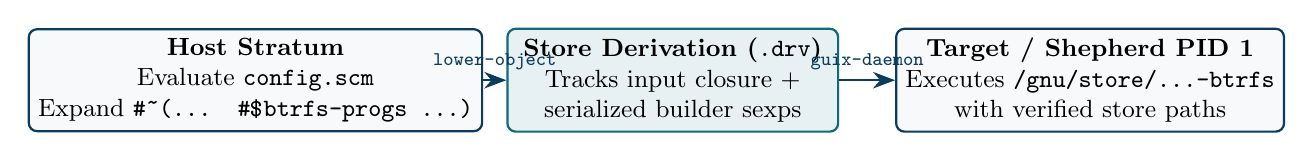
\begin{tikzpicture}[
  box/.style={draw=NavyBlue,thick,rounded corners=3pt,fill=CodeBg,align=center,minimum width=3.8cm,minimum height=1.2cm,font=\small},
  store/.style={draw=TealBlue,thick,rounded corners=3pt,fill=TealBlue!10,align=center,minimum width=4.2cm,minimum height=1.2cm,font=\small},
  arrow/.style={-{Stealth[length=2.8mm]},thick,color=NavyBlue}
]
  \node[box] (host) at (0,0) {\textbf{Host Stratum}\\Evaluate \texttt{config.scm}\\Expand \texttt{\#\textasciitilde(... \#\$btrfs-progs ...)}};
  \node[store] (drv) at (5.3,0) {\textbf{Store Derivation (\texttt{.drv})}\\Tracks input closure +\\serialized builder sexps};
  \node[box] (target) at (10.6,0) {\textbf{Target / Shepherd PID 1}\\Executes \texttt{/gnu/store/...-btrfs}\\with verified store paths};
  \draw[arrow] (host) -- node[above,font=\scriptsize\ttfamily] {lower-object} (drv);
  \draw[arrow] (drv) -- node[above,font=\scriptsize\ttfamily] {guix-daemon} (target);
\end{tikzpicture}
\end{center}

\begin{lstlisting}[language=GuileScheme]
;; Complete custom Shepherd service using G-expressions & with-imported-modules:
(use-modules (gnu)
             (gnu services)
             (gnu services shepherd)
             (gnu packages linux)
             (guix gexp))

(define %swapfile-shepherd-service
  (shepherd-service
    (provision '(swapfile))
    (requirement '(file-systems))
    (documentation "Create and activate /swapfile atomically at boot.")
    (start
      (with-imported-modules '((guix build utils))
        #~(lambda ()
            (use-modules (guix build utils))
            (let ((swap "/swapfile"))
              (unless (file-exists? swap)
                (invoke #$(file-append util-linux "/bin/fallocate") "-l" "4G" swap)
                (chmod swap #o600)
                (invoke #$(file-append util-linux "/bin/mkswap") swap))
              (invoke #$(file-append util-linux "/sbin/swapon") swap)
              #t))))
    (stop
      #~(lambda _
          (system* #$(file-append util-linux "/sbin/swapoff") "/swapfile")
          #f))))
\end{lstlisting}

\section{The 7 Layers of Guix Build Acceleration}

\begin{enumerate}
  \item \textbf{Multi-Mirror Substitutes \& Pre-Flight Check}: Configure \texttt{https://bordeaux.guix.gnu.org} and \texttt{https://ci.guix.gnu.org}, and check coverage before building via \texttt{guix weather -m manifest.scm}.
  \item \textbf{Daemon Parallelism (\texttt{--cores} vs. \texttt{--max-jobs})}: Set \texttt{--max-jobs=4} (concurrent derivations) and \texttt{--cores=8} (threads per build) so $4 \times 8 = 32$ threads saturate CPU without exhausting RAM on link steps.
  \item \textbf{In-Memory \texttt{/tmp} on \texttt{tmpfs}}: Mount \texttt{/tmp} as \texttt{tmpfs} (\texttt{flags '(no-suid no-dev)}, \texttt{options "size=16G,mode=1777"}) so \texttt{guix-daemon} unpacks and compiles tarballs entirely in RAM.
  \item \textbf{LAN Substitute Server (\texttt{guix publish})}: Run \texttt{guix-publish-service-type} with \texttt{(compression '(("zstd" 3)))} and \texttt{(advertise? \#t)} (Avahi mDNS) so laptops fetch pre-built store paths from your workstation at 2.5--10 Gbps.
  \item \textbf{Distributed Cluster Builds (\texttt{guix offload})}: Configure \texttt{/etc/guix/machines.scm} to offload heavy derivations over SSH to build servers.
  \item \textbf{Content-Addressed P2P Substitutes (GIPS)}: Mirror signed \texttt{narinfo} and \texttt{nar.zst} closures across peer nodes with cryptographic Ed25519 signature verification.
  \item \textbf{Microarchitectural SIMD Tuning (\texttt{--tune=native})}: Recompile performance-critical math/crypto packages for the host CPU's exact ISA (\texttt{znver4}, \texttt{x86-64-v3}) while keeping standard packages cached.
\end{enumerate}


% ============================================================================
% CHAPTER 4: MODULE 4 — GNU EMACS FOR LISP & GUIX ENGINEERS
% ============================================================================
\chapter{GNU Emacs for Lisp \& Guix Engineers: From First Principles to REPL Nirvana}

\section{The Emacs Mental Model: A Live Lisp Machine, Not a Text Editor}

Most newcomers approach GNU Emacs expecting a conventional text editor—a compiled binary that loads files into tabs. In reality, \textbf{GNU Emacs is a native-compiled Lisp virtual machine whose user interface happens to be text buffers}. Only the lowest-level runtime primitives (garbage collection, display rendering, subprocess I/O) are written in C; everything else—every keystroke command, window manager, Git porcelain (\texttt{magit}), and Guile IDE (\texttt{geiser})—is live Emacs Lisp executing inside a single shared address space.

\begin{center}
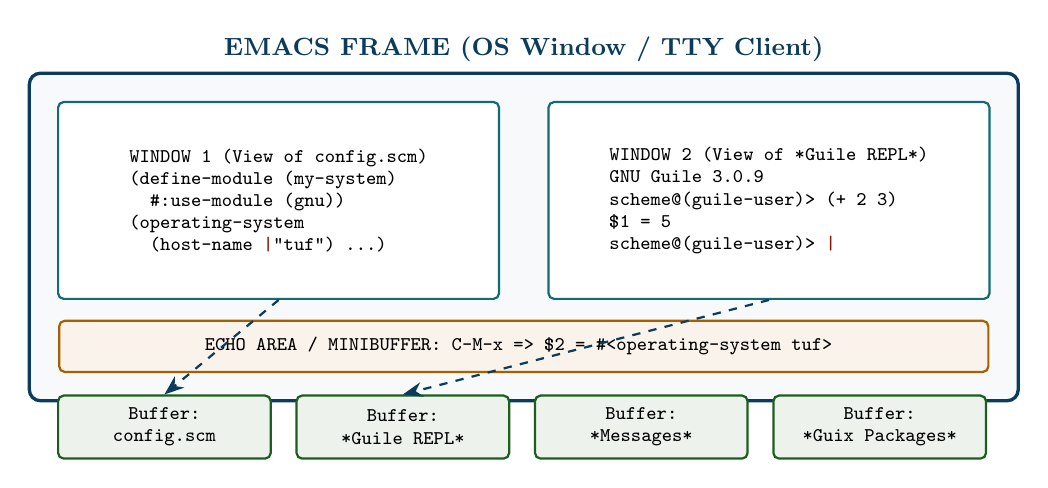
\begin{tikzpicture}[
  framebox/.style={draw=NavyBlue,very thick,rounded corners=4pt,fill=NavyBlue!3,inner sep=10pt},
  winbox/.style={draw=TealBlue,thick,rounded corners=2pt,fill=white,minimum width=5.6cm,minimum height=2.5cm,align=left,font=\ttfamily\scriptsize},
  minibox/.style={draw=AmberGold!90!black,thick,rounded corners=2pt,fill=AmberGold!8,minimum width=11.8cm,minimum height=0.65cm,align=left,font=\ttfamily\scriptsize},
  heapbox/.style={draw=ForestGreen,thick,rounded corners=2pt,fill=ForestGreen!8,minimum width=2.7cm,minimum height=0.8cm,align=center,font=\ttfamily\scriptsize},
  arrow/.style={-{Stealth[length=2.5mm]},thick,color=NavyBlue}
]
  \node[winbox] (w1) at (0,0) {
    \textbf{WINDOW 1 (View of config.scm)}\\
    (define-module (my-system)\\
    \ \ \#:use-module (gnu))\\
    (operating-system\\
    \ \ (host-name \textcolor{CrimsonRed}{|}"tuf") ...)
  };
  \node[winbox,right=0.6cm of w1] (w2) {
    \textbf{WINDOW 2 (View of *Guile REPL*)}\\
    GNU Guile 3.0.9\\
    scheme@(guile-user)> (+ 2 3)\\
    \$1 = 5\\
    scheme@(guile-user)> \textcolor{CrimsonRed}{|}
  };
  \node[minibox,below=0.25cm of $(w1.south)!0.5!(w2.south)$] (mini) {
    \textbf{ECHO AREA / MINIBUFFER:} C-M-x => \$2 = \#<operating-system tuf>
  };
  \begin{scope}[on background layer]
    \node[framebox,fit=(w1)(w2)(mini),label={[font=\bfseries\small\color{NavyBlue}]above:EMACS FRAME (OS Window / TTY Client)}] (frame) {};
  \end{scope}

  \node[heapbox,below=1.2cm of w1.south west,anchor=north west] (b1) {Buffer:\\config.scm};
  \node[heapbox,right=0.3cm of b1] (b2) {Buffer:\\*Guile REPL*};
  \node[heapbox,right=0.3cm of b2] (b3) {Buffer:\\*Messages*};
  \node[heapbox,right=0.3cm of b3] (b4) {Buffer:\\*Guix Packages*};

  \draw[arrow,dashed] (w1.south) -- (b1.north);
  \draw[arrow,dashed] (w2.south) -- (b2.north);
\end{tikzpicture}
\end{center}

\begin{itemize}[leftmargin=1.5em]
  \item \textbf{Buffer}: An in-memory Lisp object containing text, local variables, a syntax table, a keymap, and a mark ring (\texttt{C-x b} switch buffer, \texttt{C-x k} kill buffer, \texttt{C-x C-s} save file).
  \item \textbf{Window}: A tiled viewport looking into a buffer (\texttt{C-x 2} split below, \texttt{C-x 3} split right, \texttt{C-x 1} single window, \texttt{C-x o} other window). Closing a window never deletes the underlying buffer!
  \item \textbf{Frame}: An OS window or terminal screen (\texttt{emacsclient -c} graphical frame, \texttt{emacsclient -t} terminal frame) connected to your persistent \texttt{emacs --daemon}.
  \item \textbf{Point \& Mark (The Region)}: \textbf{Point} is the integer cursor offset; \textbf{Mark} (\texttt{C-SPC}) anchors the other end of the active \textbf{Region} (\texttt{M-w} copy, \texttt{C-w} kill/cut, \texttt{C-y} yank/paste).
  \item \textbf{Major vs. Minor Modes}: Every buffer has \emph{exactly one} Major Mode (\texttt{scheme-mode}, \texttt{org-mode}) and \emph{zero or more} Minor Modes (\texttt{paredit-mode}, \texttt{geiser-mode}, \texttt{flycheck-mode}). Inspect all active modes at any time with \texttt{C-h m} (\texttt{describe-mode}).
\end{itemize}

\section{Emacs Lisp (Elisp) vs. Guile Scheme: The 5 Critical Differences}

Because you configure Emacs in \textbf{Emacs Lisp} while writing Guix systems in \textbf{Guile Scheme}, you must never confuse their semantics:

\begin{center}
\begin{tabularx}{\textwidth}{lXX}
\toprule
\textbf{Dimension} & \textbf{Emacs Lisp (Elisp)} & \textbf{GNU Guile Scheme} \\
\midrule
\textbf{1. Falsiness \& \texttt{'()}} & \texttt{nil} and \texttt{'()} are \textbf{identical}. \texttt{nil} is the only false value; an empty list is falsy. & \texttt{\#f} and \texttt{'()} are \textbf{distinct}. \textbf{Only \texttt{\#f} is false}; \texttt{'()} (empty list) and \texttt{0} are \textbf{truthy}! Always use \texttt{(null? xs)}. \\
\textbf{2. Namespace (Lisp-2 vs. Lisp-1)} & \textbf{Lisp-2}: Separate function cell and value cell. Pass functions with \texttt{\#'fn}; invoke function variables via \texttt{(funcall f x)}. & \textbf{Lisp-1}: Single unified lexical namespace. Pass functions as \texttt{fn}; call function variables directly via \texttt{(f x)}. \\
\textbf{3. Scoping Rules} & \textbf{Dynamic by default} unless line 1 has \texttt{;;; -*- lexical-binding: t; -*-}. & \textbf{Lexical by default} everywhere; dynamic state uses \texttt{make-parameter}. \\
\textbf{4. Definitions \& Mutation} & \texttt{(defun f (x) ...)}, \texttt{(defvar v 1)}, \texttt{(setq x 2)}. & Unified \texttt{(define (f x) ...)}, \texttt{(define v 1)}, \texttt{(set! x 2)}. \\
\textbf{5. Tail Calls \& Loops} & No general TCO; use \texttt{dolist}, \texttt{while}, or \texttt{mapcar}. & Mandatory Tail-Call Optimization (TCO); use named \texttt{let}, \texttt{fold}, and \texttt{map}. \\
\bottomrule
\end{tabularx}
\end{center}

\section{Structural Editing (\texttt{paredit} / \texttt{smartparens}): Never Count Parentheses Again}

Experienced Lisp engineers never edit raw parenthesis characters; they manipulate balanced S-expression AST nodes directly using \textbf{Paredit} (\texttt{enable-paredit-mode}) or \textbf{Smartparens}:

\begin{lstlisting}[language=GuileScheme]
;; In every diagram below, `|' denotes Point (cursor position):

;; 1. FORWARD SLURP (`C-)'): Pulls the next right sibling INSIDE the current list
;; BEFORE: (cons* btrfs-progs |lvm2) git %base-packages
;; PRESS:  C-)  twice
;; AFTER:  (cons* btrfs-progs |lvm2 git %base-packages)

;; 2. FORWARD BARF (`C-}'): Pushes the last element OUT of the current list
;; BEFORE: (cons* btrfs-progs |lvm2 git %base-packages)
;; PRESS:  C-}
;; AFTER:  (cons* btrfs-progs |lvm2 git) %base-packages

;; 3. SPLICE (`M-s'): Dissolves the enclosing parentheses around point
;; BEFORE: (let ((x 1)) |(begin (display x) (newline)))
;; PRESS:  M-s
;; AFTER:  (let ((x 1)) |(display x) (newline))

;; 4. RAISE (`M-r'): Replaces the entire parent form with the sexp at point!
;; BEFORE: (cons* (if (laptop?) |tlp powertop) %base-packages)
;; PRESS:  M-r
;; AFTER:  (cons* |tlp %base-packages)
\end{lstlisting}

\section{Geiser, Live \texttt{guix repl} Connection, \texttt{emacs-guix} \& Complete IDE Config}

To evaluate Guix package and system definitions interactively with full access to \texttt{(gnu ...)} and \texttt{(guix ...)} modules, start a listening \texttt{guix repl} in a terminal:
\begin{lstlisting}[language=Bash]
guix repl --listen=unix:/tmp/guix-repl.sock
\end{lstlisting}
Then run \texttt{M-x geiser-connect-local RET guile RET /tmp/guix-repl.sock RET} inside Emacs. You can now evaluate top-level definitions with \texttt{C-M-x}, evaluate the preceding sexp with \texttt{C-x C-e}, expand macros inline with \texttt{C-c C-m C-e}, inspect docstrings with \texttt{C-c C-d C-d}, jump to package source definitions with \texttt{M-.}, and manage generations/store items via \texttt{M-x guix}.

\begin{protrap}[Never Load \texttt{(ice-9 readline)} Unconditionally in \texttt{\textasciitilde/.guile}]
If \texttt{\textasciitilde/.guile} activates \texttt{(ice-9 readline)} in a non-interactive pipe, Geiser's asynchronous prompt parser hangs when opening \texttt{.scm} buffers. Always set \texttt{(setq geiser-guile-load-init-file nil)} in Emacs and guard \texttt{\textasciitilde/.guile} with \texttt{(when (isatty? (current-input-port)) ...)}.
\end{protrap}

% ============================================================================
% CHAPTER 5: MODULE 5 — ORG-MODE & LITERATE SYSTEMS ENGINEERING
% ============================================================================
\chapter{Org-Mode \& Literate Systems Engineering: From Zero to Tangled OS}

\section{Outlines, GTD State Machines, Hyperlinks \& Live \texttt{\#+TBLFM:} Spreadsheets}

GNU Emacs Org-mode (\texttt{.org}) is a computable plain-text AST (\texttt{org-element}) that unifies hierarchical outlining (\texttt{TAB} subtree cycle, \texttt{S-TAB} global cycle, \texttt{M-UP}/\texttt{M-DOWN} subtree motion, \texttt{M-LEFT}/\texttt{M-RIGHT} promotion/demotion), GTD task management (\texttt{TODO} $\rightarrow$ \texttt{NEXT} $\rightarrow$ \texttt{WAIT} $\rightarrow$ \texttt{DONE}), and a live spreadsheet backed by Emacs Calc and Elisp (\texttt{\#+TBLFM:}, recalculated with \texttt{C-u C-c *}):

\begin{lstlisting}[language=OrgMode]
#+NAME: tbl-partition-budget
| Subvolume / Mount | Quota (GiB) | Quota (MiB) | Purpose                           |
|-------------------+-------------+-------------+-----------------------------------|
| /gnu/store        |          80 |       81920 | Immutable content-addressed store |
| /var/guix         |           5 |        5120 | Daemon SQLite DB & GC roots       |
| /home             |         120 |      122880 | User profiles & project worktrees |
| /tmp              |           8 |        8192 | In-RAM tmpfs build scratchpad     |
|-------------------+-------------+-------------+-----------------------------------|
| TOTAL             |         213 |      218112 | Verified allocation               |
#+TBLFM: $3=$2*1024::@6$2=vsum(@I..@II)::@6$3=vsum(@I..@II)
\end{lstlisting}

\section{Org-Babel (\texttt{ob-scheme}, \texttt{ob-shell}) \& Polyglot \texttt{:var} Pipelines}

Org-Babel executes source blocks inline via \texttt{C-c C-c}:
\begin{itemize}[leftmargin=1.5em]
  \item \textbf{\texttt{:results value}} (\emph{default}): Captures the functional return value of the final expression in the block (formatting Scheme lists-of-lists directly into Org tables).
  \item \textbf{\texttt{:results output}}: Captures \texttt{stdout} emitted during execution (\texttt{display}, \texttt{format \#t}, shell commands).
  \item \textbf{\texttt{:var x=other-block}}: Pipes tables or scalars seamlessly from a \texttt{sh} block into \texttt{python} and into \texttt{scheme}!
\end{itemize}

\section{Declarative OS Tangling (\texttt{C-c C-v t}) \& Byte-Exact Batch Tangling (\texttt{tangle.el})}

By combining \texttt{:tangle <path>}, \texttt{:mkdirp yes}, and Noweb macro expansion (\texttt{:noweb yes} with \texttt{<<component-name>>}), a single \texttt{guix-workstation.org} file generates \texttt{\textasciitilde/.config/guix/channels.scm}, \texttt{/etc/config.scm}, and \texttt{\textasciitilde/.config/guix/home.scm}:

\begin{center}
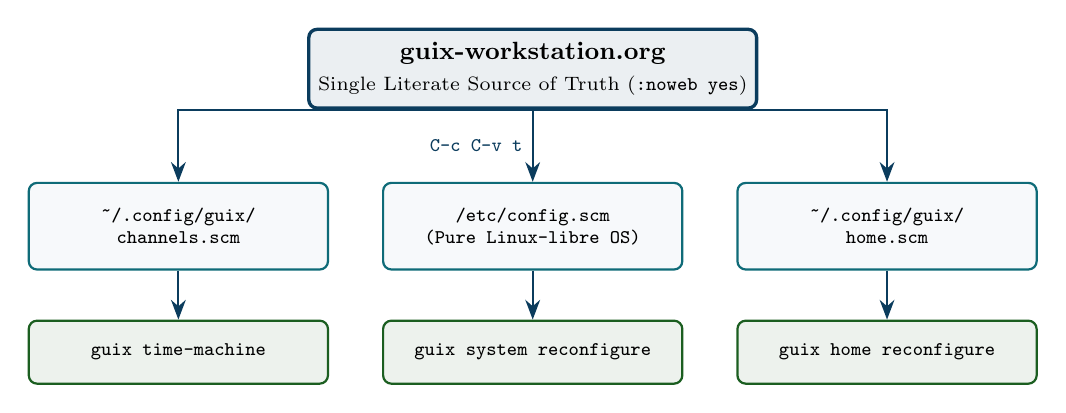
\begin{tikzpicture}[
  orgnode/.style={draw=NavyBlue,very thick,rounded corners=3pt,fill=NavyBlue!8,minimum width=5.5cm,minimum height=1.0cm,align=center,font=\bfseries\small},
  outnode/.style={draw=TealBlue,thick,rounded corners=3pt,fill=CodeBg,minimum width=3.8cm,minimum height=1.1cm,align=center,font=\ttfamily\scriptsize},
  cmdnode/.style={draw=ForestGreen,thick,rounded corners=3pt,fill=ForestGreen!8,minimum width=3.8cm,minimum height=0.8cm,align=center,font=\ttfamily\scriptsize},
  arrow/.style={-{Stealth[length=2.5mm]},thick,color=NavyBlue}
]
  \node[orgnode] (org) at (0,0) {guix-workstation.org\\{\normalfont\scriptsize Single Literate Source of Truth (\texttt{:noweb yes})}};
  \node[outnode] (chan) at (-4.5,-2.0) {\textasciitilde/.config/guix/\\channels.scm};
  \node[outnode] (sys)  at (0,-2.0)    {/etc/config.scm\\(Pure Linux-libre OS)};
  \node[outnode] (home) at (4.5,-2.0)  {\textasciitilde/.config/guix/\\home.scm};

  \node[cmdnode] (c1) at (-4.5,-3.6) {guix time-machine};
  \node[cmdnode] (c2) at (0,-3.6)    {guix system reconfigure};
  \node[cmdnode] (c3) at (4.5,-3.6)  {guix home reconfigure};

  \draw[arrow] (org.south) -- node[left,font=\scriptsize\ttfamily] {C-c C-v t} (sys.north);
  \draw[arrow] (org.south) -| (chan.north);
  \draw[arrow] (org.south) -| (home.north);
  \draw[arrow] (chan) -- (c1);
  \draw[arrow] (sys)  -- (c2);
  \draw[arrow] (home) -- (c3);
\end{tikzpicture}
\end{center}

\begin{lstlisting}[language=OrgMode]
#+title: Declarative GNU Guix Workstation (Pure FSDG / Linux-libre)
#+property: header-args :mkdirp yes :comments no

* 1. Pinned Channel (~/.config/guix/channels.scm)
#+begin_src scheme :tangle ~/.config/guix/channels.scm :tangle-mode (identity #o644)
(list (channel
        (name 'guix)
        (url "https://git.guix.gnu.org/guix.git")
        (branch "master")
        (commit "230aa373f315f247852ee07dff34146e9b480aec")
        (introduction
          (make-channel-introduction
            "9edb3f66fd807b096b48283debdcddccfea34bad"
            (openpgp-fingerprint
              "BBB0 2DDF 2CEA F6A8 0D1D  E643 A2A0 6DF2 A33A 54FA")))))
#+end_src

* 2. Modular System Blocks (/etc/config.scm)
#+NAME: os-storage
#+begin_src scheme :tangle no
(define %workstation-file-systems
  (cons* (file-system
           (device (file-system-label "GUIX_ROOT"))
           (mount-point "/")
           (type "btrfs")
           (flags '(no-atime))
           (options "compress=zstd:3,ssd"))
         (file-system
           (device (file-system-label "ESP"))
           (mount-point "/boot/efi")
           (type "vfat")
           (options "umask=0077"))
         %base-file-systems))
#+end_src

#+begin_src scheme :noweb yes :tangle /etc/config.scm :tangle-mode (identity #o644)
(use-modules (gnu) (gnu services ssh) (gnu packages shells) (guix gexp))
<<os-storage>>
(operating-system
  (host-name "guix-workstation")
  (timezone "Asia/Dubai")
  (locale "en_US.utf8")
  (kernel linux-libre)
  (bootloader (bootloader-configuration
                (bootloader grub-efi-bootloader)
                (targets '("/boot/efi"))))
  (file-systems %workstation-file-systems)
  (users (cons (user-account
                 (name "om")
                 (group "users")
                 (shell (file-append zsh "/bin/zsh"))
                 (supplementary-groups '("wheel" "netdev" "audio" "video" "kvm")))
               %base-user-accounts))
  (services (cons* (service openssh-service-type) %desktop-services)))
#+end_src
\end{lstlisting}

\begin{protrap}[Why \texttt{org-babel-tangle} Corrupts Unified Diff Patches]
Built-in \texttt{org-babel-tangle} trims leading/trailing blank lines and strips trailing whitespace, which corrupts unified \texttt{diff -u} patches stored inside Org blocks. For byte-exact tangling of OS trees and patches, parse the buffer with \texttt{(org-element-map (org-element-parse-buffer) 'src-block ...)} and write \texttt{(org-element-property :value block)} verbatim with \texttt{coding-system-for-write 'utf-8-unix}.
\end{protrap}

% ============================================================================
% CHAPTER 6: MODULE 6 — THE SEVEN GATES, 20 PRO TIPS & 7-DAY CAPSTONE
% ============================================================================
\chapter{Verification Gates, 20 Day-1 Survival Tips, Cheat Sheets \& 7-Day Capstone}

\section{The ``Seven Gates That Passed By Not Looking'' (\texttt{guix-platform-install})}

In systems engineering, a green test gate that inspects nothing is far more dangerous than no test at all, because a green check is trusted for years. During the audit of \texttt{guix-platform-install}, \textbf{seven independent gates were found reporting \texttt{[PASS]} while inspecting almost nothing}:

\begin{center}
\begin{tabularx}{\textwidth}{lXX}
\toprule
\textbf{Gate} & \textbf{How It Passed By Not Looking} & \textbf{Fail-Closed Engineering Fix} \\
\midrule
\textbf{1. Shebang Rule} & Nothing enforced it. 8 scripts had \texttt{\#!/bin/bash} (absent on Guix, where \texttt{/bin} only has \texttt{sh}), including \texttt{run-tests.sh} itself—masked because users ran \texttt{bash run-tests.sh}. & Scan every script's first line; reject \texttt{\#!/bin/bash} on Guix targets; invoke \texttt{./run-tests.sh} directly via \texttt{execve}. \\
\textbf{2. Manifest Check} & Hashed \textbf{1 file of 54}, and printed \texttt{[WARN]} on mismatch so it never gated. & Verify all $N$ files, assert \texttt{54/54 verified}, and exit non-zero on any drift. \\
\textbf{3. Unicode Check} & Used GNU-only \texttt{grep -P ... 2>/dev/null}. On macOS/BSD, \texttt{grep -P} exited \texttt{2} immediately with empty stdout, which the script treated as ``0 non-ASCII bytes found''! & Never discard \texttt{stderr} across an inverted exit check; use portable \texttt{LC\_ALL=C tr -d '[:print:][:space:]'}. \\
\textbf{4. Unit-Test Gate} & Piped \texttt{go test ./... | grep -q "ok"}, passing if \emph{one} package passed while others failed. & \textbf{Gate on exit status, never on matching text}: \texttt{if output=\$(go test ./... 2>\&1); then ...}. \\
\textbf{5. \texttt{run-tests.sh}} & Active \texttt{set -e} aborted the suite on the first deliberately tolerated legacy script failure. & Capture optional check status explicitly (\texttt{rc=0; cmd || rc=\$?}) while keeping mandatory gates strict. \\
\textbf{6. Device Tests} & Asserted ``no block devices exist,'' passing only inside an empty container and failing on real hosts. & Test parser contracts against deterministic fixture strings, never host hardware accidents. \\
\textbf{7. Eval vs. Build} & Treated ``config evaluates'' as ``config works''; \texttt{\#f} in \texttt{authorized-keys} and unbound \texttt{read-line} only crashed inside the derivation builder at build/boot time. & \textbf{Name the phase your evidence comes from}: Evaluation $\neq$ Build $\neq$ Boot $\neq$ Login. \\
\bottomrule
\end{tabularx}
\end{center}

\begin{architecturebox}[The Three Iron Laws of Verification Gates]
\begin{enumerate}
  \item \textbf{A gate that cannot say what it looked at is not a gate}: Always print explicit counts (\texttt{54 files verified}). If a glob matches \texttt{0 files}, fail immediately.
  \item \textbf{Gate on exit status, never on matching text}: Never pipe test runners into \texttt{grep -q "ok"}.
  \item \textbf{A check that cannot run must FAIL, never PASS}: Missing tools, invalid flags, or unreadable inputs must trigger an immediate non-zero exit. Prove every new gate fails by breaking the target on purpose first!
\end{enumerate}
\end{architecturebox}

\section{20 ``I Wish Someone Told Me on Day 1'' Survival Tips}

\begin{enumerate}[leftmargin=1.8em,itemsep=2pt]
  \item \textbf{Guile has no octal string escape}: \texttt{"\textbackslash 033["} is NUL + \texttt{"33["}. Always use hex \texttt{"\textbackslash x1b["}.
  \item \textbf{Multi-argument Guile shebangs require meta-switch \texttt{\textbackslash}}: Use \texttt{\#!/usr/bin/env -S guile \textbackslash} on line 1, \texttt{-e main -s} on line 2, and \texttt{!\#} on line 3.
  \item \textbf{Never mutate quoted literals \texttt{'(a b c)}}: Quoted lists reside in read-only bytecode memory; allocate mutable pairs with \texttt{(list ...)} or \texttt{(cons ...)}.
  \item \textbf{\texttt{read-line} lives in \texttt{(ice-9 rdelim)}}: Import it explicitly inside scripts and Shepherd G-expressions.
  \item \textbf{Read human prompts from \texttt{/dev/tty}, never \texttt{stdin}}: When piped (\texttt{curl ... | sh}), \texttt{stdin} is the script itself!
  \item \textbf{Silence auto-compilation noise in CLI wrappers}: Use \texttt{--no-auto-compile} or \texttt{GUILE\_AUTO\_COMPILE=0}.
  \item \textbf{Local channels and \texttt{guix time-machine} only see Git-tracked files}: Run \texttt{git add -N <file>} before building.
  \item \textbf{Mount EFI at \texttt{/boot/efi}, not \texttt{/boot}, on LVM/LUKS}: Avoids Guix GRUB module omission bug \texttt{\#44877}.
  \item \textbf{Generic VFS mount flags belong in \texttt{(flags '(no-suid no-dev no-atime))}}: Putting them inside the \texttt{(options ...)} string causes initrd \texttt{mount(2)} failures on \texttt{tmpfs}/\texttt{btrfs}.
  \item \textbf{Preserve executable bits in \texttt{local-file} with \texttt{\#:recursive? \#t}}: Plain \texttt{(local-file "script")} strips \texttt{+x} in \texttt{/gnu/store}.
  \item \textbf{OpenSSH \texttt{StrictModes} rejects \texttt{/gnu/store} symlinks in \texttt{\textasciitilde/.ssh}}: Copy \texttt{\textasciitilde/.ssh/*} files with \texttt{\#o600} permissions in a Guix Home activation G-expression.
  \item \textbf{Wrap build-side helpers in \texttt{with-imported-modules}}: Shepherd/builder G-exps need \texttt{(with-imported-modules '((guix build utils)) \#\textasciitilde(...))} to use \texttt{mkdir-p} or \texttt{invoke}.
  \item \textbf{Never leave \texttt{\#f} inside service extension lists}: Filter conditional elements with \texttt{(filter identity ...)} or splice with \texttt{,@(if cond (list item) '())}.
  \item \textbf{Guard \texttt{(ice-9 readline)} in \texttt{\textasciitilde/.guile} behind \texttt{(isatty? (current-input-port))}}: Prevents Geiser REPL hangs.
  \item \textbf{Call \texttt{(package-activate-all)} in \texttt{emacs --batch} scripts}: Batch mode skips normal post-\texttt{early-init.el} package activation.
  \item \textbf{Set \texttt{(setq org-src-preserve-indentation t)} in Emacs}: Prevents Org from corrupting \texttt{Makefile} tabs or Python indentation.
  \item \textbf{Set \texttt{\#+options: \textasciicircum:nil} in technical Org files}: Stops LaTeX/HTML export from turning \texttt{x86\_64} into subscripts.
  \item \textbf{Use \texttt{org-element-map} for byte-exact batch tangling}: Avoids \texttt{org-babel-tangle}'s blank-line trimming on patch files.
  \item \textbf{Press \texttt{C-c '} (\texttt{org-edit-special}) inside Org code blocks}: Edits the block in a dedicated full \texttt{scheme-mode} buffer with Paredit and Geiser active.
  \item \textbf{Unfreeze a stuck Emacs instantly with \texttt{pkill -SIGUSR2 emacs}}: Interrupts a runaway Elisp loop and opens \texttt{*Backtrace*} without losing unsaved buffers.
\end{enumerate}

\section{Master Quick-Reference Cheat Sheet}

\begin{center}
\begin{tabularx}{\textwidth}{llX}
\toprule
\textbf{Domain} & \textbf{Command / Key / Form} & \textbf{Purpose} \\
\midrule
\textbf{Guix CLI} & \texttt{guix time-machine -C channels.scm -- ...} & Execute any Guix command at an exact pinned channel commit. \\
\textbf{Guix CLI} & \texttt{guix shell --pure --container pkg1 pkg2} & Spawn a hermetic Linux namespace container with only listed packages. \\
\textbf{Guix CLI} & \texttt{sudo guix system roll-back} & Atomically revert OS symlink and GRUB default to previous generation. \\
\textbf{G-Exps} & \texttt{\#\textasciitilde(... \#\$pkg \#\$(file-append p "/bin/x"))} & Stage build/Shepherd code and splice store paths into target closure. \\
\textbf{Paredit} & \texttt{C-)} / \texttt{C-\}} / \texttt{M-s} / \texttt{M-r} / \texttt{M-(} & Forward slurp / forward barf / splice outer parens / raise sexp / wrap round. \\
\textbf{Geiser} & \texttt{C-M-x} / \texttt{C-x C-e} / \texttt{C-c C-d C-d} / \texttt{C-c C-m C-e} & Eval top-level define / eval last sexp / symbol docstring / macroexpand. \\
\textbf{Org Tree} & \texttt{TAB} / \texttt{S-TAB} / \texttt{M-UP/DOWN} / \texttt{M-LEFT/RIGHT} & Subtree cycle / global cycle / move subtree / promote or demote heading. \\
\textbf{Org-Babel} & \texttt{C-c C-c} / \texttt{C-c '} / \texttt{C-c C-v t} / \texttt{C-c C-e} & Execute block / edit in native major mode / tangle files / export PDF or HTML. \\
\textbf{Org-Roam} & \texttt{C-c n f} / \texttt{C-c n i} / \texttt{C-c n l} & Find or create node / insert \texttt{[[id:UUID]]} link / toggle backlinks panel. \\
\bottomrule
\end{tabularx}
\end{center}

\section{The 7-Day Capstone Engineering Curriculum}

\begin{exercisebox}[7-Day Sprint: From Bare Terminal to Literate Tangled Guix Workstation]
\begin{description}[leftmargin=1.5em,style=nextline]
  \item[Day 1 --- Guile Foundations \& Functional Pipelines:] Write a tail-recursive manifest verifier using \texttt{(srfi srfi-1)}, \texttt{(ice-9 match)}, and \texttt{define-record-type*}. \textbf{Gate:} \texttt{guild compile -Wunbound-variable -Warity-mismatch} exits \texttt{0}.
  \item[Day 2 --- Emacs, Paredit \& Live \texttt{guix repl} Connection:] Load \texttt{init-guix-ide.el}, connect Emacs to \texttt{guix repl --listen=unix:/tmp/guix.sock}, and refactor 10 nested forms using only \texttt{C-)}, \texttt{C-\}}, \texttt{M-s}, and \texttt{M-r}. \textbf{Gate:} \texttt{emacs --batch -Q -l init-guix-ide.el} exits \texttt{0}.
  \item[Day 3 --- Store Internals \& G-Expression Derivations:] Build a \texttt{computed-file} derivation using \texttt{with-imported-modules}, \texttt{\#\textasciitilde}, and \texttt{\#\$} that runs a self-check at build time. \textbf{Gate:} \texttt{guix build -f day3-gexp.scm} outputs a valid \texttt{/gnu/store} path.
  \item[Day 4 --- Custom Guix Channel \& Shepherd Service:] Create a local Git-tracked channel defining a custom package and a custom Shepherd service. \textbf{Gate:} \texttt{guix lint -L ./my-channel my-pkg} reports zero errors.
  \item[Day 5 --- Declarative Guix Home (\texttt{home.scm}):] Declare \texttt{zsh}, \texttt{\textasciitilde/.guile} (with \texttt{isatty?} guard), and an \texttt{emacs --fg-daemon} user Shepherd service. \textbf{Gate:} \texttt{guix home container home.scm -- emacs --version} exits \texttt{0}.
  \item[Day 6 --- Literate Org-Babel OS Tangling \& \texttt{org-roam}:] Unify \texttt{channels.scm}, \texttt{/etc/config.scm}, and \texttt{home.scm} inside \texttt{guix-workstation.org} with \texttt{:noweb yes} and byte-exact \texttt{tangle.el}. \textbf{Gate:} \texttt{emacs --batch -Q -l tangle.el guix-workstation.org} tangles all files cleanly.
  \item[Day 7 --- Fail-Closed Gate Suite \& Full OS VM Rehearsal:] Run \texttt{verify-guix-repo.sh} (proving it fails red when a shebang or symbol is broken, then fixing it) followed by building a bootable QEMU system VM. \textbf{Gate:} \texttt{./verify-guix-repo.sh \&\& guix time-machine -C channels.scm -- system vm /etc/config.scm} exits \texttt{0}.
\end{description}
\end{exercisebox}

\end{document}
